\documentclass[a4paper,11pt]{article}
\usepackage{ls}
\usepackage[utf8]{inputenc}
\usepackage[main=ngerman,russian]{babel}

\author{Hans-Gert Gräbe}
\title{Bericht zum Seminar am 12. Januar 2021}
\date{30.01.2021}

\begin{document}
\maketitle

\section{Zum Anliegen des Seminars}

Der Systembegriff spielt in der Informatik eine herausragende Rolle, wenn es
um Datenbanksysteme, Softwaresysteme, Hardwaresysteme, Abrechnungssysteme,
Zugangssysteme und andere Systeme geht.  Überhaupt wird die Informatik von
einer Mehrheit als die „Wissenschaft von der \emph{systematischen}
Darstellung, Speicherung, Verarbeitung und Übertragung von Informationen,
besonders der automatischen Verarbeitung mithilfe von Digitalrechnern“
(Wikipedia) verstanden.  Auch gewisse einschlägige Professionen wie etwa der
\emph{Systemarchitekt} genießen unter IT-Anwendern hohe Wertschätzung.

Die Bedeutung des Systembegriffs reicht allerdings weit über den Bereich der
Informatik hinaus -- er ist grundlegend für alle Ingenieurwissenschaften und
als \emph{Systems Engineering} mit der ISO/IEC/IEEE-15288 Norm „Systems and
Software Engineering“ auch Gegenstand internationaler Normierungs- und
Standardisierungsprozesse.  Mehr noch spielt der Systembegriff auch bei der
Beschreibung komplexer natürlicher und kultureller Prozesse -- etwa im Begriff
des \emph{Ökosystems} -- eine zentrale Rolle.

Mit dem \emph{Semantic Web} rückt die Bedeutungsanalyse digitaler Artefakte in
den Mittelpunkt, die in letzter Instanz Sprachartefakte sind und damit
ebenfalls in direktem Zusammenhang zu einem sinnvoll zu entfaltenden
\emph{Systembegriff} stehen als Grundlage jeden Verständnisses konkreter
Systeme.

Mit dem Schlagwort \emph{Nachhaltigkeit} werden schließlich komplexe
gesellschaftliche Abstimmungsprozesse angesprochen, mit denen vielfältige
Informations- und Bewertungsprobleme einhergehen. Hierbei ist die Fähigkeit
der beschreibenden Abgrenzung, Entwicklung und Steuerung von sogenannten
Systemen auf bzw. über verschiedene Governance-, Raum- und Zeitebenen hinweg
von großer Bedeutung.

Im Wintersemester 2019/20 hatten wir uns bereits mit diesem Spektrum von
\emph{Systemansätzen} (im Plural) beschäftigt, eine große Spannbreite
entsprechender Konzepte aus verschiedenen Wissenschaftsbereichen identifiziert
und diese im letzten Teil des Seminars mit Entwicklungsansätzen technischer
Systeme im Umfeld der TRIZ verglichen.  Diese Untersuchungen sollen im
aktuellen Forschungsseminar vertieft werden.

\begin{quote}
  \textbf{Ziel des Seminars} ist es, ein besseres Verständnis der
  verschiedenen Konzepte zu gewinnen, die für Gesetze, Gesetzmäßigkeiten,
  Trends und Muster der Entwicklung technischer und allgemeiner Systeme im
  Kontext der TRIZ vorgeschlagen und entwickelt wurden.
\end{quote}

Mehr zum Seminar (in deutscher Sprache) im github Repo
\begin{center}
  \url{https://github.com/wumm-project/Leipzig-Seminar}.
\end{center}

Thema des Seminars, über das hier berichtet wird, lautete \emph{Evolution
  technischer und allgemeiner Systeme bei M.S. Rubin}.  Ausgangspunkt und
Grundlage von Vortrag und Diskussion war \cite{Rubin2019}.

Dieser Text besteht aus drei Teilen,
\begin{itemize}[noitemsep]
\item meinen Anmerkungen zum Seminar,
\item dem kommentierten Chat des Seminars,
\item der von Immanuel Thoke vorbereiteten Handreichung.
\end{itemize}

\section{Anmerkungen}

M.S. Rubin beschäftigt sich schon viele Jahrzehnte mit der Frage, wie sich
Gesetze, Tendenzen und Entwicklungslinien technischer und allgemeiner Systeme
fassen lassen. Siehe dazu die Website \url{http://www.temm.ru}, die einer
\textbf{Theorie der Evolution von Materie und Modellen} gewidmet ist und damit
dem Zusammenhang zwischen materiellen Phänomenen und deren
Beschreibungsformen.  Auf der Website sind Texte von Michail Rubin und Julij
Murashkovsky zusammengetragen, wobei Rubin stärker den Zusammenhang von
materiellen und immateriellen Systemen thematisiert, Murashkovsky dagegen
stärker soziokulturelle Systeme untersucht.

In \cite{Rubin2019} werden nicht nur die Versionen von Entwicklungsgesetzen
technischer Systeme in verschiedenen TRIZ-Schulen verglichen, sondern auch
(ebenda, Abbildung 3) der Versuch unternommen, diese Gesetze zu verschiedenen
TRIZ-Werkzeugen in Beziehung zu setzen und letztlich die Verankerung der
Gesetze im Algorithmus ARIZ zu markieren.

Gesetze und Trends werden bei Rubin unterschieden, wobei letztere (Trends) als
„Haupttendenz einer Veränderung von etwas“ eingeführt werden.  Die
Unterscheidung sei „offensichtlich und wesentlich“.  Diese Differenz ist
erforderlich, denn „Modetrends“ oder „Wettertrends“ haben sicher nicht den
Charakter von Gesetzen („notwendig, substanziell, wiederkehrend“). Der
Gesetzesbegriff reicht in seinen Begründungsanforderungen tiefer, allerdings
\emph{erscheint} die Wirkung von Gesetzen nicht nur als \emph{Invarianten}
(wie etwa im Energieerhaltungssatz oder Galileis Aussage, dass Blatt und Stein
gleichschnell fallen), sondern kann sich auch als Trend (im Sinne eines
Fließgleichgewichts) manifestieren.  Darauf wurde nicht weiter eingegangen.

Die Entwicklung technischer Systeme (TS) kann sich nach Rubin auf drei Ebenen
vollziehen, als Änderung des (realweltlichen) Systems (Vollzugsform), als
Änderung des Modells (Beschreibungsform als White Box, mit Bezug auf dasselbe
realweltliche System) und als Änderung des Funktionsprinzips (Änderung der
Implementierung bei gleichbleibender Spezifikation).

Die Entwicklung eines Systems ist damit stets verbunden mit dessen
Transformation.  Da Transformationen (von einem \emph{System mit Problem} zu
einem \emph{System ohne Problem}, von einem „System, wie es ist“ zu einem
„System, wie es sein soll“) das Fundament von TRIZ sind, ist zugleich klar,
dass TRIZ wesentlich den Entwicklungsgedanken \emph{umsetzt}, womit dessen
\emph{theoretische Untermauerung} wesentlich für das TRIZ Theoriesystem ist.

Weiter wurde über \emph{Phylogenese} und \emph{Ontogenese} TS diskutiert (aucn
wenn diese bei Rubin grundsätzlich mit dem Adjektiv „systemisch“ versehen
werden).  Diese Trennung in langfristige und kurzfristige
Entwicklungsperspektiven, die in dieser aus der Biologie übernommenen
Begrifflichkeit eingefangen werden soll, rief größere Irritation hervor, auch
wenn uns die verfremdete Verwendung aus der Biologie entlehnter Begriffe im
Kontext der „technischen Ökosysteme“ bereits früher beschäftigt hat.  Ken
Kleemann wies darauf hin, dass diese Begriffe von Darwin und besonders Ernst
Haeckel\footnote{\url{https://de.wikipedia.org/wiki/Biogenetische_Grundregel}}
in der zweiten Hälfte des 19. Jahrhunderts eingeführt wurden, um
Stammesentwicklung und Individualentwicklung zueinander ins Verhältnis zu
setzen.  Basis des (biologischen) Konzepts der Phylogenese ist allerdings die
Fortpflanzung innerhalb einer Art und damit klare, realweltlich beobachtbare
Reproduktionszusammenhänge.  Epigenetische Umweltfaktoren wurden dabei
weitgehend ausgeblendet, deren Bedeutung in den letzten 50 Jahren zunehmend
deutlicher hervortritt.  (Biologische) Evolutionslinien auf höheren
Aggregationsebenen (Gattung, Familie, Ordnung, Klasse, Stamm) bewegen sich
dann nur noch auf gedanklichen Aggregaten. Die Frage, wie Rubin solche
Begriffskonstruktionen sinnvoll in eine „Welt technischer Systeme“ überträgt,
blieb weitgehend unklar, da Reproduktionszusammenhänge hier -- im Vergleich
zur Biologie -- komplett anderer Art sind, insbesondere die Behauptungen
„Gesetze sind mit der Phylogenese verbunden und Werkzeuge zur Transformation
von TS mit der Ontogenese“ und die daraus gezogene Schlussfolgerung „Das
Erkennen der Existenz von Entwicklungsgesetzen TS ist das Erkennen und
Vorhandensein phylogenetischer Prozesse in TS“ blieben unverständlich. 

Schließlich wurde diskutiert, dass der Altschullersche Begriff eines TS auf
den Begriff einer primär nützlichen Funktion (PNF) aufbaut, während
insbesondere größere Systeme \emph{multifunktionale} Systeme sind, in denen
die Auftrennung der systemischen Funktionalitäten in \emph{eine} dominante
Hauptfunktion und \emph{mehrere} Zusatz- oder Hilfsfunktionen nicht ohne
Weiteres möglich ist.

\section{Kommentierter Chat}

\subsection*{Noch einmal Ontogenese und Phylogenese}

Folie 11: Wenn TRIZ Transformation bedeutet (in einer der Boxen), dann muss es
hier um Transformation der Transformation gehen.

\begin{center}
  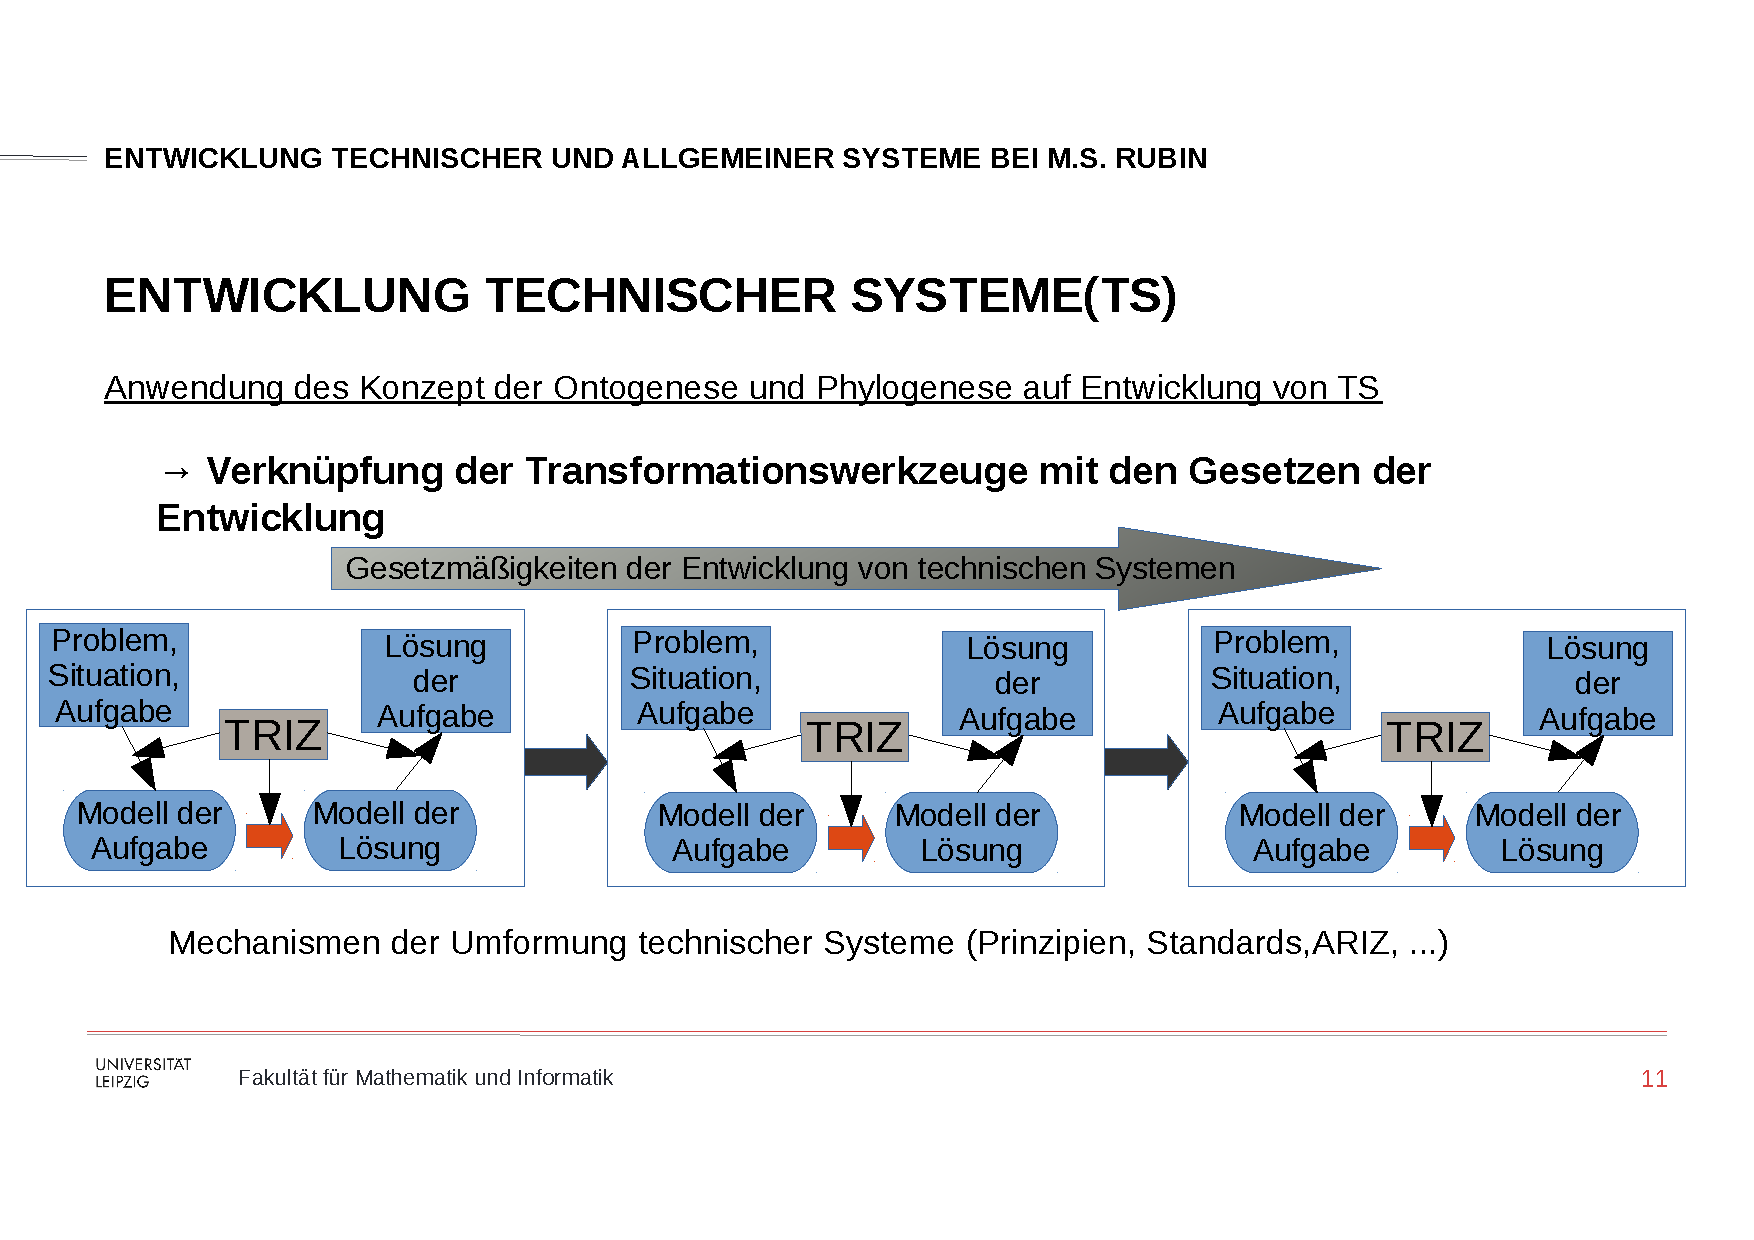
\includegraphics[width=.9\textwidth]{Folie11.pdf}
\end{center}

Nach dem Bild steht \emph{Ontogenese} für die Lösung eines Problems durch
Transformation eines TS in einem der Kästen und \emph{Phylogenese} für die
Entwicklung dieses Lösungsprozesses selbst durch Anwendung systemischer
Transformation, also für eine Transformation eines Transformationsprozesses.

\subsection*{Verschiedene Sammlungen von Gesetzen}

Rubin nennt 9 Gesetze, bei \cite{Altschuller1979} werden nur 8 Gesetze
genannt. Woher kommt die Differenz?

Das \emph{Gesetz der Dynamisierung TS} wird in \cite{Altschuller1979} und
\cite{Altschuller1980} nicht (mehr?) genannt.

\subsection*{Woher kommt die S-Kurve?}

Hinter der S-Kurve steht das mathematische Modell der \emph{logistischen
  Funktion}\footnote{\url{https://de.wikipedia.org/wiki/Logistische_Funktion}}
als Lösung eines einfachen exponentiellen Entwicklungszusammenhangs mit
Sättigungseffekt.

In \cite{Altschuller1979} und \cite{Altschuller1980} wird eine solche Kurve
als \emph{Lebenslinie} bezeichnet, wobei in \cite{Altschuller1979} im
Abschnitt 7.1 zunächst die „Lebenslinie“ entwickelt wird und danach in
Abschnitt 7.3 die Gesetze, während es in \cite{Altschuller1980} genau
umgekehrt ist.

Für Rubin ist das eher ein Muster unter mehreren möglichen und auch mehr ein
(unverbindliches) Denkmuster und kein empirisch untermauerter Fakt.  Zumal die
auf der Ordinate abgetragene Größe vage bleibt (Rubin mit Altschuller:
„Hauptmerkmale wie Kapazität, Leistung, Geschwindigkeit usw.“).

Bei Altschuller wird hier durch vertikale Abschnitte auch noch ein
Phasenmodell der Entwicklung („Kindheit“, „Reife“, „Alter“ und dann alternativ
„Stillstand“ oder „Degradierung“) hineinprojiziert.

\subsection*{MATChEM}

Folie 17 und 18 (Mythen über Grundlagen der Entwicklung Technischer Systeme)

Der Feldbegriff in der TRIZ ist ein schillerndes Konzept.

Im Welle-Teilchen-Dualismus der Physik breiten sich Wirkungen wellenförmig
aus, werden aber durch Teilchen vermittelt. So bilden etwa die Gluonen die
Austauschteilchen der starken Wechselwirkung. Ähnlich ist „ein Phonon die
elementare Anregung (Quant) des elastischen Feldes“ (Wikipedia), d.h.  bereits
in der Physik wird der Feldbegriff inflationär verwendet, wenn es darum geht,
Wirkzusammenhänge zu modellieren.  Das setzt sich in der TRIZ fort, wenn
ingenieur-technische Lösungsprinzipien konzeptualisiert werden sollen (so
steht etwa das A für „akustisches Feld“ und damit für jenes „elastische Feld“
aus der Physik).

Heute wird das oft durch I (Information) und B (Biologie) ergänzt, etwa
\cite{Belski2016}.

Es geht dabei in der TRIZ-Theorie aber auch um die Nutzung konkreter
wissenschaftlicher Effekte. Ist also eine Schnittstelle zwischen
wissenschaftlicher Erkenntnis und ingenieur-technischer Anwendung.

\section{Entwicklung technischer und allgemeiner Systeme\\ bei M.S. Rubin}
\begin{center}
  Handout von Immanuel Thoke, 10. Januar 2021
\end{center}

\subsection{Die Zyklen der Systemwissenschaft}
„Die rasante Entwicklung der Welt um uns herum macht es dringend erforderlich,
die allgemeinsten und angewandten Theorien zu entwickeln, mit denen
aufkommende Probleme aus verschiedenen Bereichen effektiv gelöst werden
können.“ \cite{Rubin2002}

Dieses Zitat lesend, fällt es schwer keinen Bezug zu klassischen
Universalgelehrten wie Leonardo da Vinci oder Gottfried Wilhelm Leibniz
herzustellen.  Ist es die vereinfachte Zugänglichkeit zu einem immer breiteren
und tieferen Wissensschatz und die Zugangsmöglichkeit zu Institutionen der
Wissenschaft für eine immer breitere Bevölkerung, die den Typos des
\emph{Universalgelehrten} zu einem verbreiteten Phänomen werden lassen?
Verlangt es neue Methoden, um dieses Wissen ordnen zu können -- eine zyklische
„Überforderung“ (im Sinne einer Obsoleszenz bisheriger Methoden), die die
Reduzierung und Strukturierung notwendig macht, um wenigstens das Gefühl zu
haben, den Überblick nicht zu verlieren -- oder legt die Materie selbst den
Blick zu systematischen Zusammenhängen frei?

Gleichzeitig, bei der Betrachtung insbesondere populärwissenschaftlicher
Medien, scheint es einen Trend zur Fokussierung auf besonders (ökonomisch)
reizvolle Themen zu geben. So gehört es mittlerweile fast zum guten Ton, sich
auch einmal mit Neurologie, Astronomie, Teilchen- oder Metaphysik beschäftigt
zu haben. Wenngleich die ursprüngliche Expertise auf den ersten Blick wenig
mit den bearbeiteten Themen zu tun hat, werden Muster erkannt, die zur
infradiziplinären Untersuchung der Spezifika und möglicher Generika leiten.
Wenngleich in der öffentlichen Diskussion regelmäßig populärwissenschaftliche
Analogien mit Fachtermini verwechselt werden, ist der Aspekt einer
interparadigmatischen strukturellen Kreativität ein Zeichen der „systemischen
Inbezugnahme“ vor allem naturwissenschaftlicher Forschungsfelder -- man denke
nur einmal an die Entwicklung neuronaler Netze.

Rubin unterscheidet zunächst grob zwischen materiellen und immateriellen
Systemen. Die Kategorie der materiellen Systeme reicht dabei von anorganischen
und organischen (physikalisch-chemischen), lebenden
(biophysikalisch-chemischen) bis hin zu sozialen und soziotechnischen
Systemen.  Für ihn haben all diese Systeme „einheitliche Entwicklungsgesetze“
\cite{Rubin2002}. Immaterielle Systeme behandeln „die Entstehung von Mensch,
Vernunft und Zivilisation“ \cite{Rubin2006} und damit „Systeme wie
Wissenschaft, Kunst, Religion, Technologie, Sprache und viele andere“
\cite{Rubin2006}, wobei unklar bleibt, ob dies als eine Art „metaphysisches
System“ zu begreifen ist oder beschreibt, wie sich Menschen in einem
ontologischen System verhalten. Er framt immaterielle Systeme unter dem
Begriff der \emph{Kultur} und weist gleichzeitig auf die Problematik der
normativen Prägung derjenigen Gesetze aufmerksam, die gemeinhin als
Naturgesetze bezeichnet werden. Er bringt dazu Beispiele wie „Weltbilder als
Schlachtfeld von Theorien und Menschen“, die Revidierung der
Phlogiston-Theorie und diverse Beispiele der „Strukturinduktion“ durch Gesetze
als „notwendige, substanzielle, nachhaltige, wiederkehrende Beziehung zwischen
Phänomenen in Natur und Gesellschaft“ -- wobei Natur hier wohl eher im
übertragenen Sinne als Obersystem und allgemeingültiger Handlungsrahmen
verstanden werden muss -- wie bspw. antike Kalender, Traditionen oder
juristische Handlungsrahmen.

Die Verbindung von Transformationswerkzeugen und Gesetzen der Entwicklung von
Systemen ist ein zentraler Aspekt seiner Methodologie. Das erscheint zunächst
trivial, wird aber als wesentliches Charakteristikum von Systemwissenschaften
verstanden \cite{Kleemann2020}: Dass dies aber insbesondere für die
Transformationsschritte der Modellierungsphase und nicht zwangsläufig auf die
Methoden der Implementierung übertragbar ist, wurde im Seminar ausführlich
diskutiert. Gleichzeitig offenbart dies jedoch die Doppeldeutigkeit des
Begriffs \emph{Entwicklung}, und es stellt sich die Frage, inwieweit die
Einheit von System und Methode als Einheit von Theorie und Praxis tatsächlich
relevant sein kann, wenn man die intersubjektiven Begriffssemantiken
betrachtet.

\subsection{Analogismen infradisziplinärer Systematik}
„Was Physiker ein Gesetz nennen, nennen Mathematiker eine Vermutung.“ (Scott
Aaronson)

Vielleicht ist es schlicht naheliegend, dass sich Rubin eines biologischen
Terminus bedient, um Muster in der Entwicklung von Systemen mittels Ontogenese
und Phylogenese zu charakterisieren und kategorisieren. Schließlich lässt sich
die Biologie historisch als eine frühe interdisziplinäre Systemwissenschaft
begreifen, die sich spätestens seit Mendel und Darwin mit Merkmalsbeschreibung
und Strukturentwicklung beschäftigte.

Jedoch stellt sich die Frage, inwieweit sich Fachtermini grundsätzlich auf
andere Disziplinen übertragen lassen oder ob in deren Anwendung auf fachfremde
Zusammenhänge eine terminologische Differenz zum Ausdruck kommt, da sich der
fachfremden Materie im Abgleich der terminologischen Information lediglich
asymptotisch genähert werden kann. Mit Analogien geht das Spiel schnell
auf. Das Mammut kann mit der Pferdekutsche und der Elefant mit dem
Verbrennerauto gleichgesetzt werden. Die Orthologierelationen, die sich aus
phylogenetischen Informationen herleiten lassen, können auf die
Maschinenelemente des PKWs übertragen werden. Diese Begriffsanalogie führt zu
einer Strukturäquivalenz und damit zu einem Problem. Die Strukturäquivalenz
gilt nur innerhalb der Fächergrenzen. Für den Wissenstransfer ist jedesmal
eine Übersetzungsleistung notwendig. Spätestens wenn es juristisch gesicherte
Definitionen braucht, um die geplanten Systeme alltagstauglich zu machen,
verschwinden objektive Grenzen erster Ordnung und damit die Einheit von
soziotechnischen Systemen und deren Methodik im langfristigen Zeitfenster.

Bekanntlich ist die Justizia jedoch blind, und vielleicht hilft an dieser
Stelle nur das Spannungsfeld der Heuristik, die sich auch in der Luhmannschen
Systemtheorie niederschlägt. Insofern die Grammatiken der Individuen, deren
kommunikative Inferenzen sich nicht als bijektives Mapping darstellen lassen,
irrationale Vorgänge in Form erwartungskonformer Institutionen
rationalisieren, formen sie ihr eigenes „objektives“ Gesetz zweiter Ordnung,
an das sie sich halten müssen, um einander zu verstehen. Indem man sich
gegenseitig auf einen gemeinsamen Wortlaut verständigt und die approximierte
Zuordnung validiert, anstatt Widerspruch in vermeintlich mangelnder Exaktheit
zu suchen, können Nuancen der individuellen Auslegung anhand des Kontextes im
Prozess reinterpretiert werden, sofern die Rückkopplung anhand des dynamischen
gesellschaftlichen Kontexts mit einbezogen werden.

In diesem Sinne gilt: Die Bedeutung eines Begriffs \emph{ist} dessen Gebrauch.

\begin{thebibliography}{yyy}
\bibitem{Altschuller1979} Genrich S. Altschuller (1979).
  \foreignlanguage{russian}{Творчество как точная наука}.  Deutsch 1983:
  \emph{Erfinden -- (k)ein Problem}.
\bibitem{Altschuller1980} Genrich S. Altschuller, Alexander B. Seljutsky
  (1980). \foreignlanguage{russian}{Крылья для Икара}. Deutsch 1983:
  \emph{Flügel für Ikarus}.
\bibitem{Belski2016} Iouri Belski, Pavel Livotov, Oliver Mayer (2016). Eight
  Fields of MATCEMIB Help Students to Generate More Ideas. Procedia CIRP
  39:85-90.  DOI \texttt{10.1016/j.procir.2016.01.170}
\bibitem{Kleemann2020} Ken P. Kleemann (2020). Dialektik der kreativen
  Innovation.  In: Erfinderschulen, TRIZ und Dialektik. Rainer Thiel zum
  90. Geburtstag.  Rohrbacher Manuskripte, Heft 20. ISBN 9783751983228.
\bibitem{Rubin2002} Michail S. Rubin (2002).  \foreignlanguage{russian}{О
  теории развития материальных систем (ТРМС).} (Über eine Theorie der
  Entwicklung materieller  Systeme). \\
  \url{http://www.temm.ru/ru/section.php?docId=3878}.
\bibitem{Rubin2006} Michail S. Rubin (2006). \foreignlanguage{russian}{Принцип
  захвата и многообразия в развитии систем.} (Das Prinzip des Einfangens und
  Mannigfaltigkeiten in der Entwicklung von Systemen).\\
  \url{http://www.temm.ru/ru/section.php?docId=3433#2}.
\bibitem{Rubin2019} Michail S. Rubin (2019).  \foreignlanguage{russian}{О
  связи комплекса законов развития систем с ЗРТС} (Zum Zusammenhang zwischen
  dem Komplex der Entwicklungsgesetze allgemeiner Systeme und den
  Entwicklungsgesetzen technischer Systeme).  Manuskript, 06.11.2019.
\end{thebibliography}

\end{document}
